%%%%%%%%%%%%%%%%%%%%%%%%%%%%%%%%%%%%%%%%%%%%%%%%%%%%%%%%%%%%%%%%%%%%%%%%%%%%%%%%%%%%%%%%%%%%%%%%%%%%
% NN neuron
% Adapted from: http://tex.stackexchange.com/questions/132444/diagram-of-an-artificial-neural-network

\RequirePackage{luatex85}
\documentclass[border=0.5mm]{standalone}
\usepackage[a-1b]{pdfx}
\usepackage{tikz}
\usetikzlibrary{calc}
% \usetikzlibrary{decorations.pathmorphing}
% \usetikzlibrary{decorations.markings}
\usetikzlibrary{decorations.pathreplacing}
\usetikzlibrary{chains}
\usetikzlibrary{arrows} % deprecated, should migrate away from o-latex, someday...

\usepackage{xcolor}
% Colors from https://styleguide.duke.edu/color-palette/

% These are the official colors, and they cannot be modified by the program (ie changing the opacity or saturation)
\definecolor{Duke Blue}{HTML}{001A57}
\definecolor{Blue Devil Blue}{HTML}{0736A4}

% These are the official recommendations for colors to go with the two official Duke colors. PMS is the Pantone Matching system index, so you can search the color to see what it should look like
\definecolor{PMS Black 3}{HTML}{262626}
\definecolor{PMS Cool Gray 11}{HTML}{666666}
\definecolor{PMS Cool Gray 7}{HTML}{B5B5B5}
\definecolor{PMS Cool Gray 3}{HTML}{E5E5E5}
\definecolor{Light Gray}{HTML}{F5F5F5}

% Blues
\definecolor{PMS 294}{HTML}{003366}
\definecolor{PMS 3015}{HTML}{235F9C}
\definecolor{PMS 3005}{HTML}{0680CD}

% Oranges
\definecolor{PMS 166}{HTML}{D75404}
\definecolor{PMS 1805}{HTML}{CC3300}
% \definecolor{PMS 157}{HTML}{F09905}

% Other
\definecolor{PMS 392}{HTML}{728302} % dark green
\definecolor{PMS 390}{HTML}{A1B70D} % light green
\definecolor{PMS 123}{HTML}{FFD960} % light yellow
\definecolor{PMS 2617}{HTML}{993399} % nice violet


\begin{document}
\resizebox{15cm}{!}{%
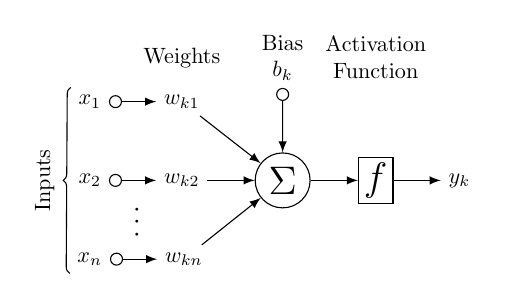
\begin{tikzpicture}[x=1.2cm, y=1.2cm]
  \pgfmathsetmacro{\textscale}{0.8}

  \tikzstyle{annot} = [scale=\textscale,text centered]
  \tikzstyle{labeltext} = [scale=0.8,text centered] % its the same at 0.8 but is now easily changeable


  \tikzstyle{circ} = [draw, circle, inner sep=2pt,
  font=\Large, % Sigma size
  join = by -latex]

  \tikzstyle{squa} = [draw, inner sep=2pt,
  font=\Large,
  join = by -latex]

\begin{scope}[start chain=2,node distance=6mm]

\node[on chain=2, annot]
  (x2) {$x_{2}$};
\node[on chain=2,join=by o-latex, annot]
  {$w_{k2}$};
\node[on chain=2,circ] (sigma)
  {$\displaystyle\Sigma$};

\node[squa, on chain=2] (actfunc) {$f$};

% \node[annot, on chain=2,join=by -latex,xshift=0.3cm] (output) {$y$};
\node[annot, on chain=2,join=by -latex] (output) {$y_{k}$};

\begin{scope}[start chain=1]
\node[on chain=1, annot] at (0,1cm)
  (x1) {$x_{1}$};
\node[on chain=1,join=by o-latex, annot]
  (w1) {$w_{k1}$};
\end{scope}

\begin{scope}[start chain=3]
\node[on chain=3, annot] at (0,-1cm)
  (xn) {$x_{n}$};
\node[annot, on chain=3, join=by o-latex]
  (wn) {$w_{kn}$};

\end{scope}

\node[labeltext, yshift=0.7cm] at (w1) (labely) {Weights};
% \node[labeltext] at (labely-|output) {\parbox{2cm}{\centering Output}};
\node[labeltext] at (labely-|actfunc) {\parbox{2cm}{\centering Activation\\Function}};

\node[labeltext] at (labely-|sigma) (b) {\parbox{1cm}{\centering Bias\\$b_{k}$}};

\draw[-latex] (w1) -- (sigma);
\draw[-latex] (wn) -- (sigma);
\draw[o-latex] (b) -- (sigma);

\draw[decorate,decoration={brace,mirror}] (x1.north west) -- node[labeltext, pos=0.5, xshift=-0.125cm, anchor=south,rotate=90] {Inputs} (xn.south west);

% \path (x2) -- node[red,pos=0.5,rotate=90,yshift=-0.55cm]{\ldots} (xn); % By hand pos
\node[rotate=90] at ( $(x2)!0.5!(wn)$ ) {\ldots}; % calc pos

\end{scope} % end chain 2, place here so all the weights line up in x

\end{tikzpicture}
} % end resizebox
\end{document}
